\chapter{Larvitrampas}
En esta sección se presentan las consideraciones a tener en cuenta para la construcción, instalación y revisión de larvitrampas.

\section{Construcción de larvitrampas}
Las larvitrampas son, dispositivos artificiales creados con el fin de simular el habitad de mosquitos de forma controlada. El diseño más simple (\figref{fig:anexo-construccion-larvitrampas})
es una sección radial de una llanta llena de agua \cite{world2009dengue, manualControlArg2009}.

\begin{figure}[!htbp]
\centering
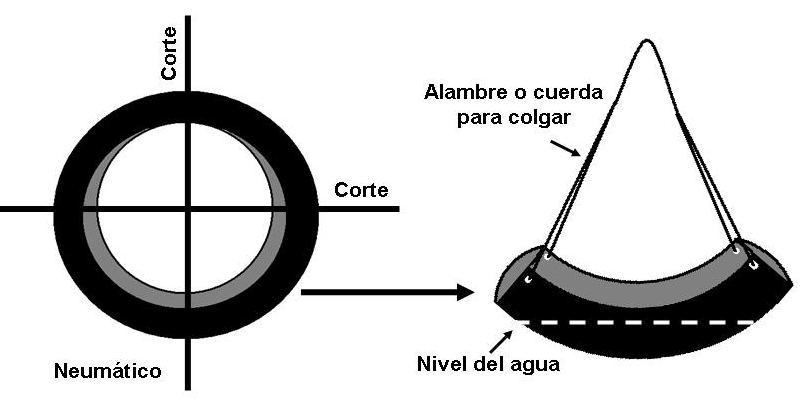
\includegraphics[width=0.9\textwidth]{anexos/graphics/construccion-larvitrampa.png}
\caption{\label{fig:anexo-construccion-larvitrampas} Diseño de una larvitrampa(Tomado de
\cite{manualControlArg2009}).}
\end{figure}

Las llantas o neumáticos son considerados como criaderos de alto riesgo
\cite{bisset2008distribucion, manrique1998desarrollo, ulloa1996abundancia}, donde, la
supervivencia y la  duración del ciclo de vida en neumáticos son menores a los reportados para
otros tipos de contenedores \cite{manrique1998desarrollo}. Esto resalta la importancia de los
neumáticos como criaderos y blanco para el control del vector del dengue
\cite{manrique1998desarrollo, ulloa1996abundancia}.

Las llantas deben cortarse en 4 partes, donde cada sección radial corresponde a una larvitrampa,
donde dependiendo de el lugar de su instalación podría optase por un diseño colgante
(\figref{fig:anexo-disenho-1}), mediante una soga o alambre, o un diseño fijo
(\figref{fig:anexo-disenho-2}), en el suelo mediante un pedazo de madera. Se debe establecer un
mecanismo de etiquetado, que facilite su identificación, de forma que se pueda asociar la
información obtenida a una larvitrampa.

\begin{figure}[!htbp]
    \centering
    \begin{subfigure}[b]{0.45\textwidth}
        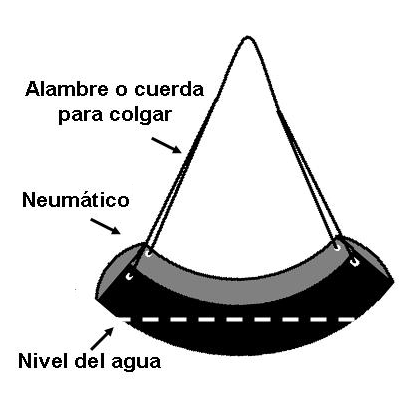
\includegraphics[width=0.9\textwidth]{anexos/graphics/disenho-1.png}
        \caption{\label{fig:anexo-disenho-1} Diseño de una larvitrampa colgante (Tomado de
        \cite{manualControlArg2009}).}
    \end{subfigure}
    ~~~~
    \begin{subfigure}[b]{0.45\textwidth}
        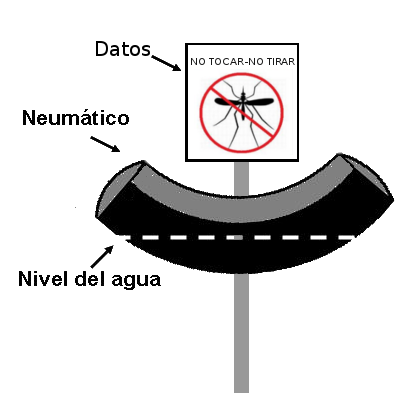
\includegraphics[width=0.9\textwidth]{anexos/graphics/disenho-2.png}
        \caption{\label{fig:anexo-disenho-2} Diseño de una larvitrampa fija al suelo.}
    \end{subfigure}
    \caption{\label{fig:disenhos-larvitrampas} Diseños de larvitrampas dependiendo del lugar de instalación.}
\end{figure}

Antes de la utilización de la larvitrampa, ésta debe cepillarse y flamearse, luego mantenerla
sumergida en agua durante no menos de tres días, para asegurarse que el agua no contenga residuos
de sustancias que puedan actuar como larvicida \cite{manualControlArg2009}. De esta manera,
además, se garantiza la destrucción de algún huevo del mosquito que estuviese previamente en el
neumático o en larvitrampas ya utilizadas \cite{manualControlArg2009}.

Las larvitrampas, construidas de neumáticos, permiten transformar estos criaderos de alto riesgo
en una herramienta para el control del vector del dengue mediante el reciclaje.

\section{Consideraciones para la instalación}
Deben ser instaladas a una altura de 50 centímetros de la base del suelo, donde la ubicación debe
ser seleccionada de forma a protegerla de la luz directa del sol, el aire, y la lluvia de forma
que la instalación se realice en lugares con luz media o completamente a la sombra
\cite{manualControlArg2009}. No deben ubicarse en las cercanías de depósitos de agua. Además hay
que evitar su instalación en lugares completamente pavimentados, u otros que tengan mucha
refracción de la luz \cite{manualControlArg2009}.

\begin{figure}[!htbp]
    \centering
    \begin{subfigure}[b]{0.45\textwidth}
        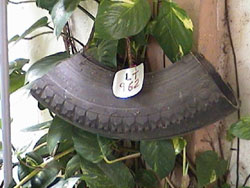
\includegraphics[width=0.9\textwidth]{anexos/graphics/ej1-larvitrampa.png}
        \caption{\label{fig:anexo-disenho-1}Ejemplo de una larvitrampa instalada de forma colgante.}
    \end{subfigure}
    ~~~~
    \begin{subfigure}[b]{0.45\textwidth}
        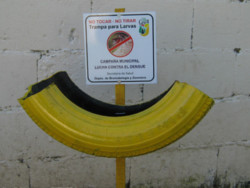
\includegraphics[width=0.9\textwidth]{anexos/graphics/ej2-larvitrampa.png}
        \caption{\label{fig:anexo-disenho-2} Ejemplo de una larvitrampa instalada fija al suelo.}
    \end{subfigure}
    \caption{\label{fig:instalacion-larvitrampas} Ejemplos de instalación de una larvitrampas.}
\end{figure}

Hay que considerar que las larvitrampas deben estar visibles y atractivas para la ovipostura, a
hembras del mosquito, además hay que protegerla de los niños y animales domésticos (perros, gatos,
roedores, etc.). Deben facilitar la inspección visual del agua insitu o que permita transferir
fácilmente su contenido a otro recipiente para su análisis.

\section{Periodo y formas de revisión}
El periodo de revisión de las larvitrampas no debe ser superior a 7 días para evitar la aparición
de mosquitos adultos. Hay que tener en cuenta que la tasa de desarrollo de los mosquitos depende
de la temperatura, por lo que en verano, las condiciones tienden a ser más favorables para el
desarrollo de esta especie. Motivo por el cual el periodo de inspección debe calcularse en base a
las tasas de desarrollo correspondientes a la temperatura, a fin de evitar que alguna de ellas se
transformen en criaderos de adultos.

El contenido debe vaciarse cuidadosamente, para que no quede ninguna larva fija en las paredes de
la larvitrampa, en un recipiente adecuado para realizar la inspección. En caso de ser positivas,
se registra como tal y las larvas serán colectadas en tubos para ser enviadas al laboratorio para
su determinación taxonómica \cite{manualControlArg2009}.

Luego, el dispositivo se debe lavar y acondicionar para su reutilización siguiendo las
especificaciones descritas anteriormente.
